\documentclass[times, utf8, zavrsni]{fer}
\usepackage{booktabs}
\usepackage{graphicx}
\usepackage{caption}
\usepackage{subcaption}

\begin{document}

% TODO: Navedite broj rada.
\thesisnumber{6461}

% TODO: Navedite naslov rada.
\title{Profiliranje autora na društvenim mrežama}

% TODO: Navedite vaše ime i prezime.
\author{Ivan Lovrenčić}

\maketitle

% Ispis stranice s napomenom o umetanju izvornika rada. Uklonite naredbu \izvornik ako želite izbaciti tu stranicu.
\izvornik

% Dodavanje zahvale ili prazne stranice. Ako ne želite dodati zahvalu, naredbu ostavite radi prazne stranice.
\zahvala{}

\tableofcontents


\chapter{Uvod}


\indent U posljednjih nekoliko godina načini ljudske komunikacije doživljavaju novu paradigmatsku promjenu. Neizbježna prisutnost interneta te svih njegovih usluga stvorila je priliku za nove globalne načine komunikacije. Najpopularniji, te trenutno najutjecajniji alat, upravo su društvene mreže. U posljednjih nekoliko godina, rast korisnika društvenih mreža raste gotovo eksponencijalnom brzinom. Podaci iz 2018. godine govore kako je broj aktivnih korisnika interneta dosegnuo nevjerojatnih 4,38 milijardi, što iznosi približno oko 57\% svjetske populacije.\footnote{https://www.smartinsights.com/social-media-marketing/social-media-strategy/new-global-social-media-research/} Taj postotak, u pojedinim razvijenim dijelovima svijeta, doseže gotovo 95\%, a još nevjerojatniji podatak jest da većina aktivnih korisnika koristi internet isključivo radi komunikacije putem društvenih mreža.

Kako svijet postaje sve više digitaliziran i načini komunikacije polako prelaze na novije medije, javlja se potreba za metodama pomoću kojih je moguće kvalitetno i efikasno profilirati sve brojnije korisnike. Brojne tehnološke firme, poput Facebooka,\footnote{https://www.facebook.com/} Youtubea,\footnote{https://www.youtube.com/} pa čak i one koje ne spadaju u standardan opis društvene mreže, imaju potrebu za kvalitetnim određivanjem karakteristika njihovih korisnika. Razlozi za profiliranjem su brojni te variraju od želje za blokiranjem nepoželjnih korisničkih ponašanja do personaliziranih oglasa za svakoga korisnika. No, za potpunu obradu sve većeg broja korisnika i informacija potrebno je obraditi nevjerojatno velike količine podataka. Upravo taj sve veći broj podataka zahtijeva promišljeni pristup te pomoć računala.

Interakcijom računala i prirodnog jezika korisnika bavi se obrada prirodnog jezika (engl. \textit{natural language processing}). Uz obradu prirodnog jezika, za temeljito rješavanje ovog problema potrebno je još koristiti vještine i metode iz umjetne inteligencije (engl. \textit{artifical intelligence}) te računalne lingvistike (engl. \textit{computational linguistics}). Područja primjene obrade prirodnog jezika su brojna te uključuju odgovaranje na pitanja (engl. \textit{question answering}), određivanje teme (engl. \textit{topic detection}), određivanje sentimenta ( engl. \textit{sentiment analysis}) te, dio koji ćemo detaljnije obrađivati u ovome radu, analizu autora (engl. \textit{author analysis}).

Ovaj se rad bavi profiliranjem korisnika Twittera\footnote{https://twitter.com/} uz pomoć metoda strojnog učenja. Rad se sastoji od tri odvojena zadatka. Prvi zadatak je određivanje spola korisnika, drugi je određivanje dobi te treći je određivanje intenziteta pet različitih psiholoških značajki. U sljedećih nekoliko poglavlja bit će detaljno objašnjeni modeli, metode evaluacije te podaci koji su korišteni u ovom radu. Na samome kraju bit će prezentiran zaključak te potencijalni budući rad na ovoj temi. 


\chapter{Srodni radovi}


Porastom popularnosti društvenih mreža, profiliranje autora je postala sve važnija i atraktivnija lingvistička disciplina. S pojavom organiziranih natjecanja poput PAN profiliranje autora (engl. \textit{PAN Author Profiling}) \footnote{https://pan.webis.de/tasks.html-task-authorship-profiling}sve više ljudi saznaje za ovo relativno neistraženo područje. PAN je serija znanstvenih događanja i natjecanja iz područja tekstualne forenzike i stilometrije. Brojni radovi se objavljuju svake godine te se bilježi sve veći napredak u kvalitetnom profiliranju korisnika. 

Tema i sami zadatak ovog rada su preuzeti sa PAN 2015\footnote{https://pan.webis.de/clef15/pan15-web/author-profiling.html} gdje je službeni zadatak bio određivanje spola, dobi i psiholoških značajki autora. Na preuzetu temu je objavljeno mnoštvo radova te svi bilježe određene uspjehe. Česta poveznica među radovima je velik naglasak na stilometrijskim značajkama, kojima se pokušava što bolje specificirati stilove autora te samim time omogućiti modelima veću prediktivnu moć. Također, u radovima je česta praksa razdvajanje skupova značajki, odnosno rastavljanje značajki sadržaja teksta od značajki stila autora, kako bi se kvalitetnije demonstrirao utjecaj pojedinog skupa značajki na kvalitetu modela \citep{rangel2013}. 

Za značajke sadržaja teksta pretežito je korišten frekvencija pojma - inverzna frekvencija dokumenta (engl. \textit{Term Frequency-Inverse Document Frequency}) faktor (TF-IDF faktor), što je učestalo korištena procedura za određivanje informativnosti svake od riječi u korpusu \citep{notebook2015}. Osim faktora TF-IDF uspješni rezultati dobiveni su s vrećom riječi (engl. \textit{bag-of-words,BoW}), n-gramovima (engl. \textit{n-grams}) te vektorima termina (engl. \textit{term vectors}) \citep{rangle2015}. 

S druge strane, stilometrijske značajke se konstantno razvijaju i prilagođavaju novim načinima komunikacije. U službenom zadatku s PAN 2015 svi autori su bili korisnici društvene mreže Twitter te se stoga pokazalo da stilometrijske značajke dosta ovise o platformi na kojoj korisnik objavljuje. Primijećeno je da su česte uporabe ključnih riječi (engl. \textit{hashtag,\#}) snažna indikacija za predviđanje pojedinih psiholoških značajki autora. Osim ključnih riječi, ostale značajke specifične za Twitter poput \textit{retweetanja} i označavanje ostalih korisnika u objavi također su imale veliku korelaciju s autorovim psihološkim profilom \citep{rangle2015}.

U ovom radu korištena su dva zasebna skupa značajki. Prvi skup značajki odnosi se na značajke sadržaja teksta, no u odnosu na čestu praksu u radovima, u ovome radu korištena je metoda vektorske reprezentacije riječi (engl. \textit{word embeddings}) za razliku od faktora TF-IDF i ostalih korištenih značajka sadržaja teksta. Drugi skup značajki su stilometrijske značajke koje su djelomično preuzete iz već obrađenih radova te su testirane u kombinaciji sa značajkama sadržaja teksta. Značajke su korištene za učenje u modelu za određivanje spola, dobi te intenziteta psiholoških značajki autora. 


 
\chapter{Strojno učenje}

Strojno učenje grana je umjetne inteligencije koja se bave oblikovanjem algoritama koji svoju učinkovitost poboljšavaju na temelju empirijskih podataka. Sastoji se od skupa metoda i algoritama kojima možemo postići da računalo nauči rješavati određeni problem, a da ga eksplicitno ne isprogramiramo za to rješenje. Naime, algoritam strojnog učenja stvara model koji je definiran parametrima čija se vrijednost određuje iz podataka na kojima se algoritam uči. Nakon procesa učenja model se može nalaziti u stanju prenaučenost (engl. \textit{overfitting}), podnaučenosti (engl. \textit{underfitting}) ili u optimalnom stanju. Prenaučenost se događa kada se model previše prilagodi podacima na kojima se uči te zbog toga loše generalizira na neviđenim podacima.\footnote{https://en.wikipedia.org/wiki/Overfitting} S druge strane, podnaučeni model nije se dovoljno prilagodio podacima na kojima je treniran te ponovo ima problem s generalizacijom na primjerima koje još nije vidio\footnote{https://www.datarobot.com/wiki/underfitting/}. U optimalnom slučaju model se naučio generalizirati na podacima koji su mu pruženi te može kvalitetno predviđati na podacima s kojima se još nije susreo. U domeni strojnog učenja postoji nekoliko različitih tipova problema koji se rješavaju, od kojih su najpoznatiji nadzirano učenje (engl. \textit{supervised learning}) i nenadzirano učenje (engl. \textit{unsupervised learning}).\newline


\begin{figure}[h]
	\centering
	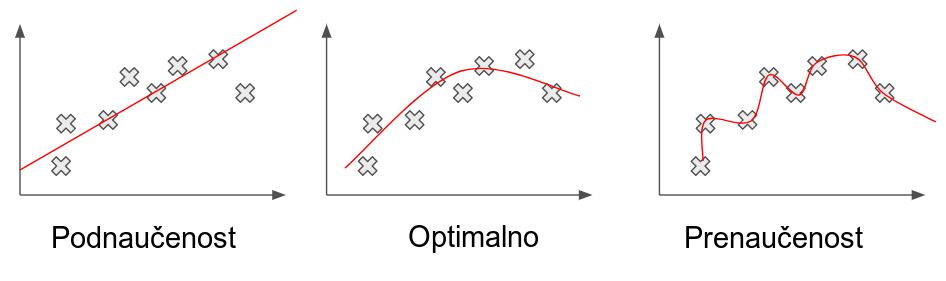
\includegraphics[width=\linewidth]{slika2.png}
	\caption{Prikaz različitih modela ovisno o naučenosti \protect \footnotemark}
\end{figure}


\footnotetext{https://pythonmachinelearning.pro/wp-content/uploads/2017/09/Overfitting.png}



Algoritmi i metode nadziranog učenja bave se izgradnjom matematičkih modela koji za pruženi skup podataka oblika $(x,y)$, pri čemu je $x$ vektor značajki, a $y$ oznaka klase kojoj pripada vektor, grade funkciju  preslikavanja $y = f(x)$. Naknadno, nadzirano učenje možemo podijelit na klasifikaciju (engl. \textit{classification}) i regresiju (engl. \textit{regression}) \citep{love2002}.
Glavna distinkcija između klasifikacije i regresije je u izlazu modela. Oba modelu primaju vektor značajki x na ulaz, no izlaz u klasifikacijskom modelu je diskretna, a regresijskom kontinuirana vrijednost.

S druge strane, kod nenadziranog učenja skup podataka se sastoji samo od ulaza, odnosno podaci dolaze samo u obliku x vektora značajki, dok uz to nije priložena y oznaka klase. Algoritmi pronalaze vezu među podacima te stvaraju smislene strukture u dobivenom skupu podataka. Najkorištenije metode unutar ovih algoritama su grupiranje (engl. \textit{clustering}), smanjenje dimenzionalnosti (engl. \textit{dimensionality reduction}) te procjena gustoće (engl. \textit{density estimation}).\newline


 
\begin{figure}
	\centering
	\begin{subfigure}{.5\textwidth}
		\centering
		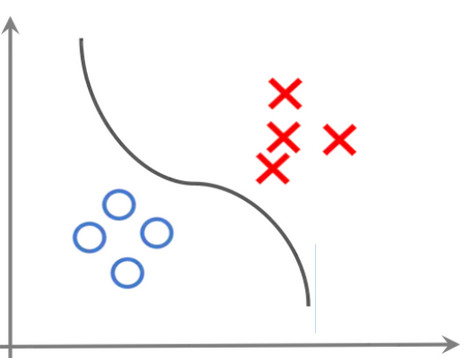
\includegraphics[width=\linewidth]{foto1}
		\caption{Nadzirano učenje}
		\label{fig:sub1}
	\end{subfigure}%
	\begin{subfigure}{.5\textwidth}
		\centering
		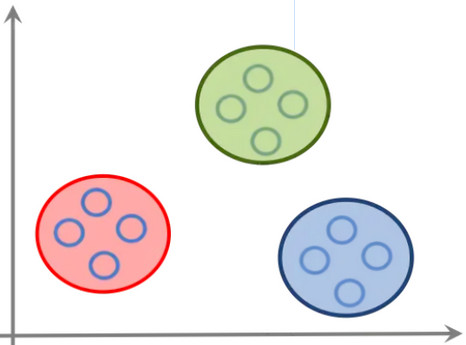
\includegraphics[width=\linewidth]{foto2}
		\caption{Nenadzirano učenje}
		\label{fig:sub2}
	\end{subfigure}
	\caption{Usporedba nadziranog i nenadziranog učenja \protect\footnotemark}
	\label{fig:test}
\end{figure}

\footnotetext{https://cdn-images-1.medium.com/max/1600/1*6mPnd6tEA4EsYD1f72hGkA.png}
\newpage

\section{Stroj potpornih vektora}

U domeni nadziranog strojnog učenja postoji velik opus različitih algoritama i metoda za klasifikaciju i regresiju podataka. S obzirom na prirodu zadataka ovog rada, potreban nam je moćan klasifikator koji dobro surađuje s alatima za obradu prirodnog jezika. Jedan od najmoćnijih alata s tim opisom je stroj potpornih vektora. (engl. \textit{Support vector machine, SVM})\footnote{https://en.wikipedia.org/wiki/Support-vector\_machine} 

SVM je skup metoda u domeni nadziranog strojnog učenja. Njegova nadmoć, u odnosu na ostale algoritme, leži u specifičnom načinu modeliranju podataka koje obrađuje. Naime, model SVM-a podatke prikazuje kao točke u hiperprostoru  te pokušava povući optimalnu hiperravninu koja će razdvojiti podatke s obzirom na njihove oznake. Udaljenost između točaka koje pripadaju različitim klasama naziva se margina te je SVM-ov cilj povući hiperravninu koja će maksimizirati marginu, odnosno udaljenost između različitih klasa \citep{fradkin2006}. Cijeli proces leži na matematičkoj interpretaciji potpornih vektora koji se definiraju kao vektori na rubovima ravnine,odnosno kao marginalno najbliži podaci različitih klasa. Primjer rada SVM-a te odabira optimalne hiperravnine prikazan je na slici 3.3.\newline


\begin{figure}[h]
	\centering
	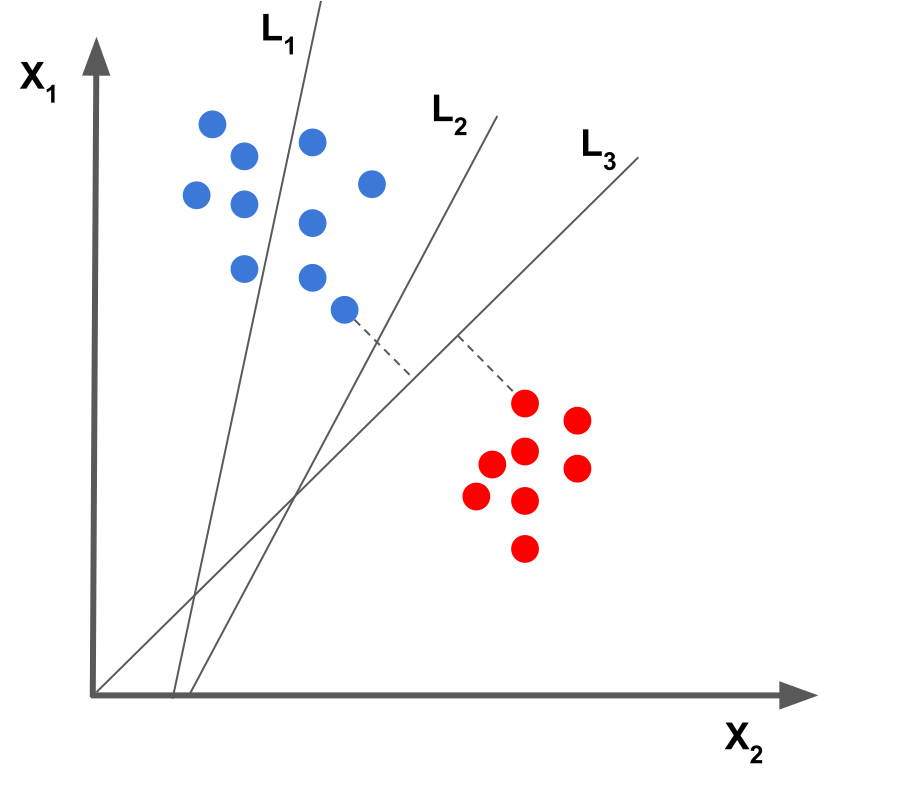
\includegraphics[width=8cm]{svm1}
	\caption{Oba pravca L3 i L2 razdvajaju različite klase, no pravac L3 ima maksimalnu marginu, odnosno najveću udaljenost između različitih klasa.\protect\footnotemark}
\end{figure}

\footnotetext{https://upload.wikimedia.org/wikipedia/commons/2/20/Svm\_separating\_hyperplanes.png}

\newpage


SVM je po definiciji linearan klasifikator, no ponekad skup podataka nije linearno razdvojiv. U slučaju linearne nerazdvojivosti SVM ima dva načina rada: metodu čvrste margine (engl. \textit{hard-margine}) i metodu meke margine (engl. \textit{soft-margine}).

Metoda čvrste margine koristi se u slučajevima kada je skup podataka linearno razdvojiv. U tom slučaju SVM može odrediti dvije paralelne hiperravnine koje razdvajaju dvije različite oznake podataka. Prilikom povlačenja paralelnih hiperravnina, SVM uvijek cilja na osiguravanje maksimalne margine, odnosno najveće udaljenosti između dviju paralelnih hiperravnina. Primjer metode čvrste margine prikazan je na slici 3.4.\newline

\begin{figure}[h]
	\centering
	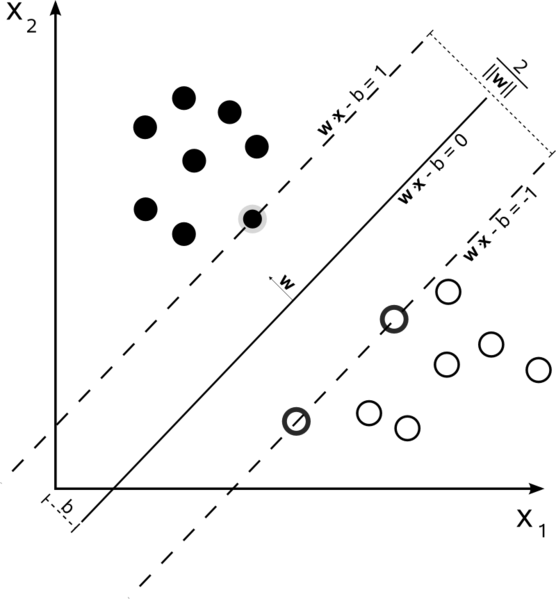
\includegraphics[width=10cm, height=10cm]{svm2}
	\caption{Metoda čvrste margine u SVM-u \protect\footnotemark}
\end{figure}

\footnotetext{https://www.researchgate.net/profile/Tapan\_Bagchi/publication/263716081/figure/fig1/AS:392444068810765@1470577365764/The-Hard-Margin-SVM-in-the-X1-X2-feature-space.png}

S druge strane, metoda meke margine koristi se kada ravninom nije moguće razdvojiti vektore različitih klasa. U slučaju meke margine u obzir uzimamo određenu pogrešku prilikom presijecanja prostora te se stoga uvodi funkcija gubitka prostora (engl. \textit{hinge loss function}):

\begin{equation}
	max(0,1-y_{i}(\overrightarrow{w} * \overrightarrow{x_{i}} - b))
\end{equation}

Funkcija gubitka prostora nam služi kao pomoćni alat za svojevrsno ispravljanje algoritma ukoliko vektor značajki $x_{i}$ ostane na neispravnoj strani margine.\footnote{https://en.wikipedia.org/wiki/Hinge\_loss} Vrijednost $y_{i}$ predstavlja oznaku klase te nam je također cilj osigurati da vektor značajki $x_{i}$ ostane uparen s ispravnom oznakom klase $y_{i}$. Varijabla $\overrightarrow{w}$ predstavlja normalu hiperravnine za koju računamo funkciju gubitka prostora, dok $b$ predstavlja konstantu hiperravnine.

\begin{equation}
	[\frac{1}{n} \sum_{i=1}^{n} max(0,1-y_{i}(\overrightarrow{w} * \overrightarrow{x_{i}} - b))] + \lambda * \|w\|^2
\end{equation}
\newline

Spajajući izraz 3.1 sa SVM-ovom ciljem maksimiziranja margine modela, dobiva se izraz 3.2 čijom minimizacijom optimiziramo ispravnu klasifikaciju te maksimalnu moguću marginu modela. Parametar $\lambda$ određuje vezu između zahtjeva za povećanjem margine i zahtjeva da vektor značajki $x_{i}$ se nalazi na ispravnoj strani margine. Stoga, za dovoljno male vrijednosti $\lambda$, drugi dio izraza postaje zanemariv te se algoritam počinje ponovo ponašati kao SVM sa metodom čvrste margine ukoliko je skup podataka moguće linearno razdvojiti. \newline

U posebnim slučajevima SVM može linearno nerazdvojive skupove podataka obraditi na drugačiji način. Naime, u slučajevima nelinearne klasifikacije SVM pomoću transformacijske funkcije, još zvane jezgrena funkcija (engl. \textit{kernel function}), transformira prostor skupa podataka u višedimenzijski prostor u kojem je moguća višedimenzijska linearna podjela \citep{kernel}. Jezgrena funkcija ovisi o dva hiperparametra C i $\gamma$ te je poželjno, u slučajevima kad se koristi, provesti optimizaciju kako bi klasifikator radio na optimalan načinu. Primjer načina rada jezgrene funkcije prikazan je na slici 3.5.

\begin{figure}[h]
	\centering
	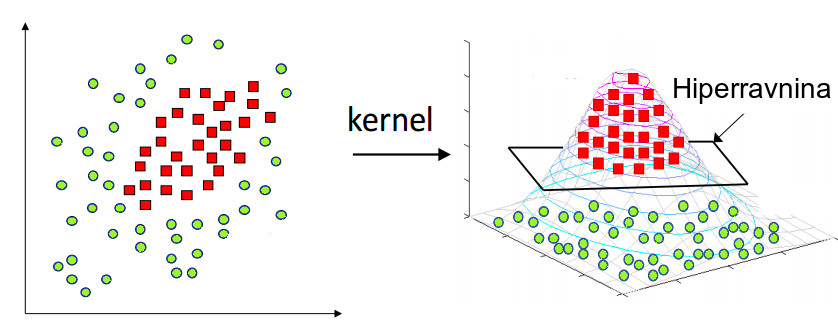
\includegraphics[width=11cm]{kernel}
	\caption{Prebacivanje u višedimenzijski prostor u kojem je moguće linearna raspodjela\protect\footnotemark}
\end{figure}

\footnotetext{https://blog-c7ff.kxcdn.com/blog/wp-content/uploads/2017/02/kernel.png}


Osim za probleme binarne klasifikacije, SVM je iznimno moćan višeklasni klasifikator. Glavna metoda prilikom rješavanja višeklasnog problema jest svođenje višeklasne klasifikacije na nekoliko binarnih klasifikacija \citep{svm_multiclass}. Jedna od najčešćih metoda za takav način rješavanja problema jest pomoću izgradnje više binarnih klasifikatora. Sa više klasifikatora zatim možemo klasificirate oznake na način da jednu oznaku klasificiramo u odnosu na sve ostale (engl. \textit{one-versus-all}) ili klasificiranjem par po par oznaka (engl. \textit{one-versus-one}).
 U \textit{one-versus-all} metodi traži se oznaka koja će imati najveći izlaz, odnosno za koju će klasifikator dobiti najbolju točnost u odnosu na sve ostale oznake. U metodi \textit{one-versus-one} gleda se takozvani ukupan rezultat svih klasifikacija te se uzima oznaka koja je ostvarila najbolji rezultat u svim međusobnim klasifikacijama.
 
 \begin{figure}[h]
 	\centering
 	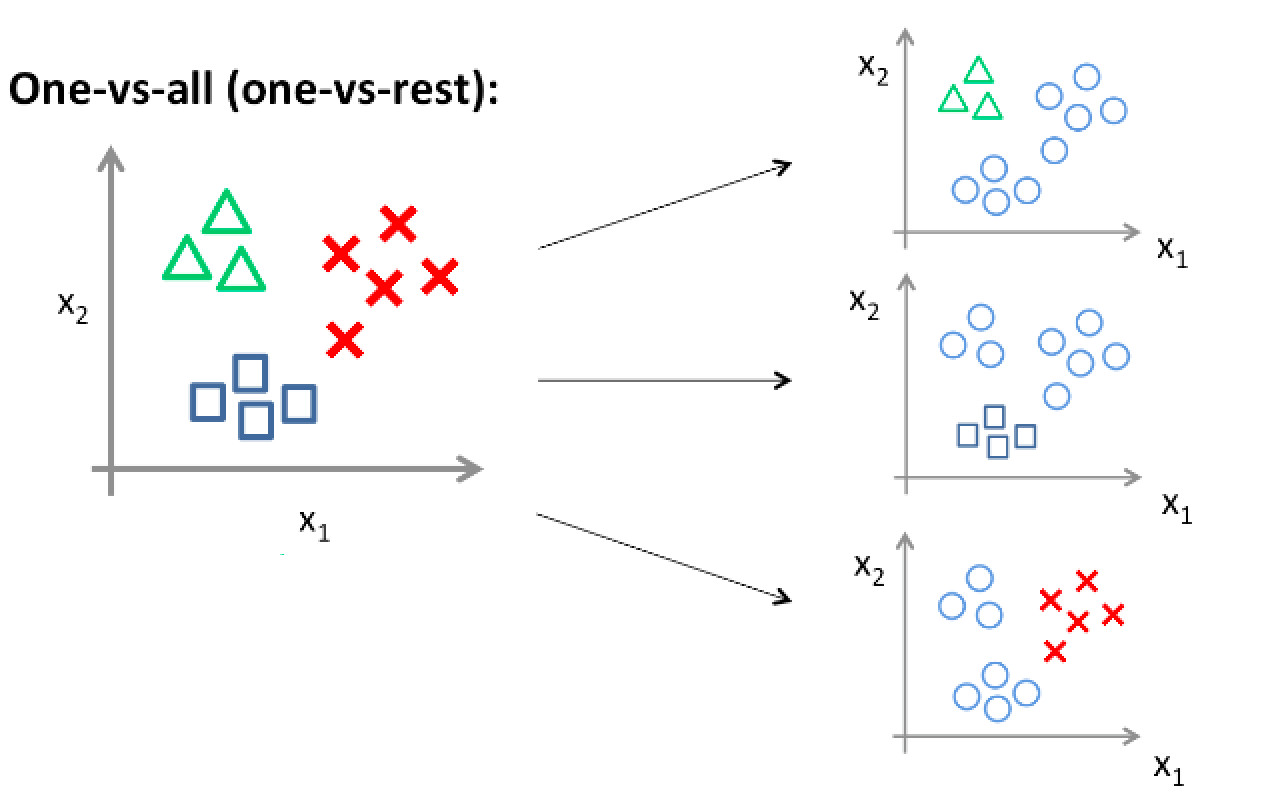
\includegraphics[width=11cm]{multiclass}
 	\caption{Prikaz načina rada one-versus-all metode\protect\footnotemark}
 \end{figure}

\footnotetext{https://houxianxu.github.io/images/logisticRegression/4.png}

Uz klasifikacijske probleme, SVM je opremljen opusom alata za modeliranje regresijskih problema. Princip rada regresije je usko povezan sa radom SVM klasifikatora. I dalje je cilj osiguravanja maksimalne margine, no u slučaju regresije izlaz je realan broj što dodatno otežava osiguranje maksimalne margine. U regresiji uvodimo marginalnu toleranciju $\epsilon$ unutar koje prihvaćamo sva predviđanja modela. Cilj regresijskog algoritma jest minimiziranje sljedećeg uvjeta: 

$$\frac{1}{2}\left\lVert w\right\rVert^2$$.

Odnosno, minimiziranje norme vektora normale $\overrightarrow{w}$ uz uvjet da: 

$$ y_{i} - \langle w,x_{i} \rangle - b \leq \epsilon $$
$$ \langle w,x_{i} \rangle + b - y_{i} \leq \epsilon$$

gdje je $x_{i}$ vektor značajki sa oznakom klase $y_{i}$, a $b$ je konstanta specifična za ravninu s kojom presijecamo prostor. Predikcija izlaza za taj par $(x_{i},y_{i})$ se mora nalaziti unutar marginalnog intervala određenog sa parametrom $\epsilon$ kako bi se izlaz smatrao valjanim. Pobliže objašnjen način rada regresije u SVM-u je objašnjeno na slici 3.7. Svi crveno obojani podaci se ne smatraju valjanima, jer nisu unutar marginalne granice $\epsilon$. 

 \begin{figure}[h]
	\centering
	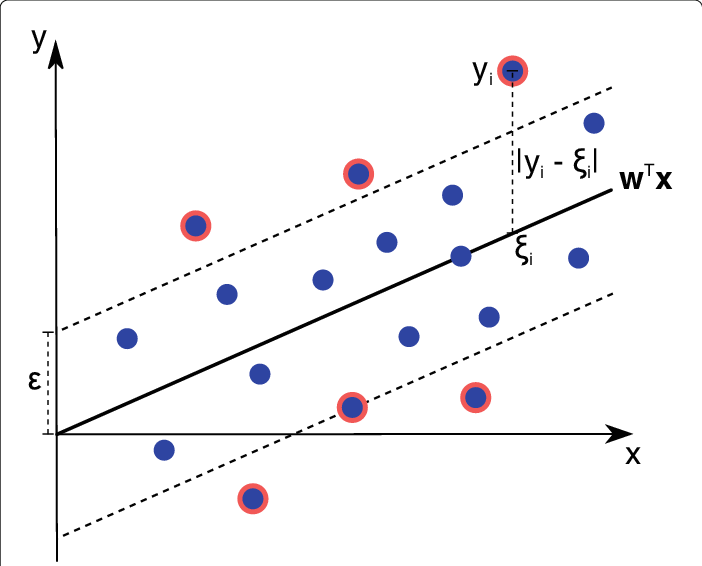
\includegraphics[width=7cm]{regression}
	\caption{Prikaz načina rada SVR-a \protect\footnotemark}
\end{figure}

\footnotetext{https://cdn-images-1.medium.com/max/1600/1*rs0EfF8RPVpgA-EfgAq85g.jpeg}



\newpage
\section{Logistička regresija}

U bogatom opusu alata nadziranog učenja, logistička regresija (engl. \textit{logistic regression}), također pripada popisu moćnijih algoritama strojnog učenja. Logistička regresija, iako ime upućuje na drugačije, je klasifikacijski model strojnog učenja. Definira se kao diskriminativni model koji za izlaz ima vjerojatnosno tumačenje te je zbog toga i vjerojatnosni model.

Uvođenjem nelinearne funkcije \textit{f} može se priopćiti linearan regresijski model:

\begin{equation}
	h(x) = f(w^T x+w_{0})
\end{equation}

Funkcija f naziva se još i aktivacijska funkcija, a zadatak te funkcije je da linearnu funkciju preslika u jedinični interval. Za logističku regresiju je tako definirana logistička ili sigmoidalna funkcija \citep{logistic}:

\begin{equation}
	\sigma(w^T x+w_{0}) = \frac{1}{1+\textit{exp}(-w^T x-w_{0})}
\end{equation}\newline

\begin{figure}[h]
	\centering
	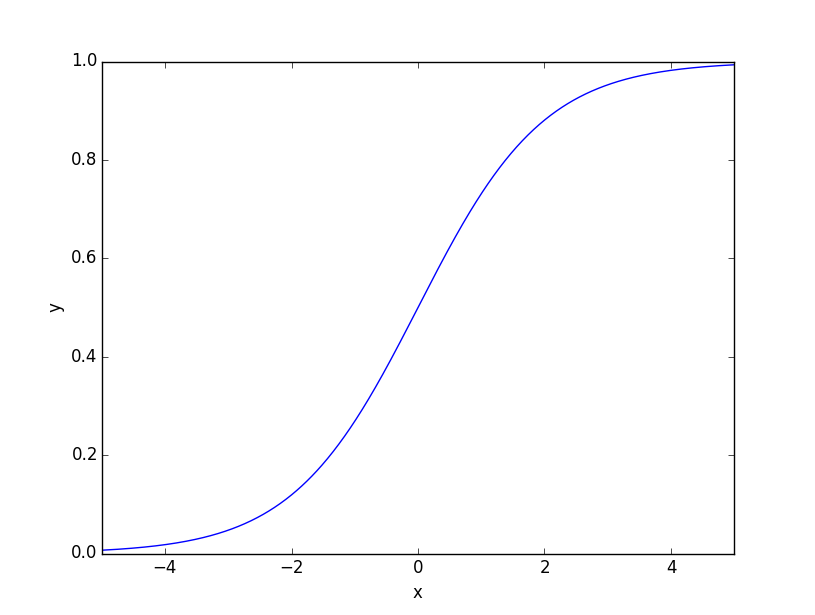
\includegraphics[width=9cm,height=7cm]{sigmoidbla}
	\caption{Prikaz sigmoidalne funkcije \protect\footnotemark}
\end{figure}

\footnotetext{https://nathanbrixius.files.wordpress.com/2016/06/sigmoid.png}

Sigmoidalna funkcija prikazana na slici 3.7 koristi se zbog svoje mogućnosti preslikavanja vrijednosti u interval između 0 i 1, što je pogodno u klasifikacijskim zadacima za prikazivanje vjerojatnosti.

\newpage

Na slici 3.8 imamo vizualni prikaz u razlici rada između SVM-a i logističke regresije. Na primjeru je vidljivo kako SVM traži maksimalnu marginu između dvije različite klase, dok na desnoj sličici vidimo kako logistička regresija traži samo maksimalnu točnost te joj margina nije prioritet u klasifikaciji podataka. \newline

Učenje modela logističke regresije se tako svodi na određivanje parametra $w^T$, a optimizacija parametara svodi se na minimizaciju funkcije pogreške na skupu za treniranje:

\begin{equation}
	E(w^T|D) = - \sum_{i=1}^{N} \{ \textit{y}^{(i)} \textit{ln}(\textit{h}(\textit{x}^{(i)})) + (1-\textit{y}^{(i)}) \textit{ln}(1-\textit{h}(\textit{x}^{(i)})) \} + \frac{\lambda}{2} \sum_{j=1}^{n} |w_{j}|^q
\end{equation}

\noindent gdje je $ \frac{\lambda}{2} \sum_{j=1}^{n} |w_{j}|^q$ regularizacijski izraz kojim se povećava funkcija pogreške za složenije modele te se time smanjuju slučajevi prenaučenosti modela \citep{logistic}.

\begin{figure}
	\centering
	\begin{subfigure}{.5\textwidth}
		\centering
		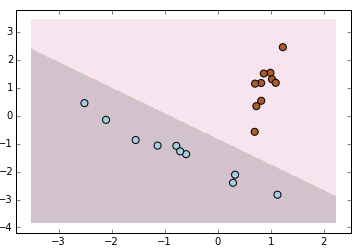
\includegraphics[width=\linewidth]{bla1}
		\caption{SVM}
		\label{fig:sub1}
	\end{subfigure}%
	\begin{subfigure}{.5\textwidth}
		\centering
		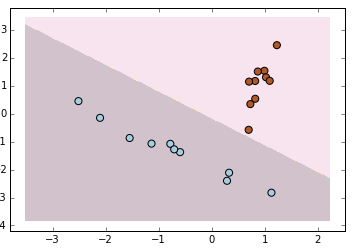
\includegraphics[width=\linewidth]{bla2}
		\caption{Logistička regresija}
		\label{fig:sub2}
	\end{subfigure}
	\caption{Usporedba binarne klasifikacije između SVM i logističke regresije \protect\footnotemark}
	\label{fig:test}
\end{figure}

\footnotetext{https://github.com/jsnajder/MachineLearningTutorial/blob/master/Machine\%20Learning\%20Tutorial.ipynb}




\chapter{Podaci i model}
\section{Skup podataka}

Skup podataka korišten za potrebe eksperimenata ovog rada preuzet je s PAN 2015 \citep{description_paper}\footnote{https://pan.webis.de/clef15/pan15-web/author-profiling.html}. Cilj njihovog službenog zadataka je bio profiliranje autora po dobi, spolu te predviđanje intenziteta psiholoških značajki u spektru od -0.5 do 0.5. Skup psiholoških značajki sastoji se od: \textit{ekstrovertnost, stabilnost, otvorenost, savjesnost i ugodnost} (engl. \textit{extrovertness, stable, open, conscientious, agreeable}).
 
Preuzeti skup podataka sastoji se od skupa za učenje (engl. \textit{training dataset}) i skupa za testiranje (engl. \textit{test dataset}). Skup za učenje se sastoji od 152 autora te je za svakog autora izdvojeno 100 jedinstvenih \textit{tvitova}. S druge strane, skup za testiranje modela sastoji se od 142 autora za koje je također za svakog odvojeno 100 jedinstvenih \textit{tvitova}.

U želji za optimiranim modelima, preuzeti skup podataka zahtijevao je određene preinake. Za temeljito optimiziranje modela potreban je skup podataka za provjeru (engl. \textit{validation dataset}) s kojim optimiramo hiperparametre modela strojnog učenja. U ovom slučaju manualno je podijeljen skup za testiranje u dva skupa omjera 60:40, od kojih većinski skup postaje skup za provjeru, a manji skup poprima ulogu novog skupa za testiranje.


\begin{table}[h!]
	\centering
	\begin{tabular}{||c |c | c||} 
		\hline
		Skup podataka & Broj autora & Broj tvitova \\ [0.5ex] 
		\hline\hline
		Trening & 152 & 15200 \\ 
		Provjera & 82 & 8200 \\
		Test &  70 & 7000  \\
		\hline
	\end{tabular}
	\caption{Raspodjela broja autor i tvitova po skupovima podataka}
	\label{Table:1}
\end{table}



\section{Model}

U sklopu ovog rada razvijena su tri različita modela: binarni klasifikator spola, višeklasni klasifikator dobi te klasifikator intenziteta psiholoških značajki autora. Svi modeli su implementirani u programskom jeziku Python,\footnote{https://www.python.org/} verzija 2.7.12. Python je odabran zbog velikog opusa dostupnih alata iz domene strojnog učenja te alata iz domene obrade prirodnog jezika \citep{python}. Za potrebe ovog rada korištene su Python-knjižice poput scikit-learna,\footnote{https://scikit-learn.org/stable/} iz kojih su preuzeti algoritmi nadziranog strojnog učenja poput već objašnjenih SVM-a i logističke regresije.

Za razvoj modela korištena su dva skupa značajki. Prvi skup značajki su značajke sadržaja teksta, a drugi dio su stilometrijske značajke usmjerene na zahvaćanje stila autora teksta. Značajke su podijeljene u dvije kategorije radi lakšeg praćenja utjecaja vrste značajki na prediktivnu sposobnost modela \citep{rangel2013}.




\subsection*{Značajke sadržaja teksta} 

Prva skupina značajki su značajke sadržaja teksta. Ovim značajkama želimo izvući čim više semantičkog značenja iz samog teksta te odrediti utjecaj sadržaja teksta u profiliranju autora. U ovome radu je korištena metoda vektorske reprezentacije riječi (engl. \textit{word embeddings}) pomoću predtreniranih vektora (engl. \textit{pre-trained vectors}) \citep{notebook2017}. Najpopularniji alati s ovim opisom su Googleov Word2Vec,\footnote{https://code.google.com/archive/p/word2vec/} GloVe (Global Vectors)\footnote{https://nlp.stanford.edu/projects/glove/} te Facebookov fastText.\footnote{https://fasttext.cc/} U ovom radu su korištena sva tri alata uz cilj da se otkrije najbolja metoda vektorske reprezentacije za ovaj specifičan zadatak profiliranja autora.

\subsubsection{Word2Vec}

Word2vec je skupina povezanih modela koji se koriste za razvoj vektorske reprezentacije riječi. Radi se o plitkim, dvoslojnim neuronskim mrežama koje su posebno naučene za rekonstrukciju lingvističkog konteksta iz riječi. Kao ulaz u mrežu Word2vec prima ogroman korpus teksta te iz njega proizvodi višedimenzijski vektorski prostor. Svaka riječ iz korpusa je predstavljena vlastitim i specifičnim vektorom čije se dimenzije nerijetko se broje u stotinama \citep{word2vec}. \newline



\begin{figure}[h]
	\centering
	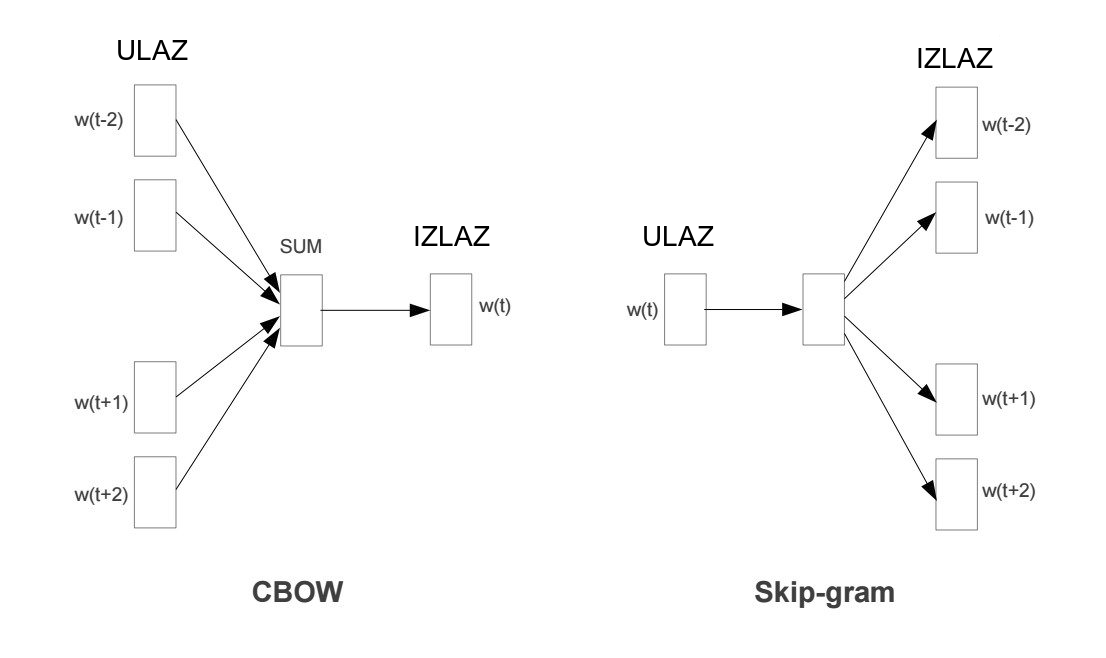
\includegraphics[width=12cm]{slika10}
	\caption{Prikaz rada word2veca sa CBOW i skip-gramom \protect\footnotemark}
\end{figure}

\footnotetext{https://i.imgur.com/vNYiUZi.jpg}


U postupku učenja modela Word2veca koristi se jedna od dviju metoda:

\begin{itemize}
	\item kontinuirana vreća riječi (engl. \textit{continuous bag-of-words, CBOW})\footnote{https://en.wikipedia.org/wiki/Bag-of-words\_model}
	\item kontinuirani skip-gram (engl. \textit{continouous skip-gram})
\end{itemize}

	
U metodi CBOW model predviđa trenutnu riječ iz konteksta ostalih riječi koje ju okružuju. S druge strane, u metodi skip-gram model koristiti trenutačnu riječ za predviđanje konteksta riječi koje bi ju trebale okruživati \citep{word2vec2}. Kontekstni prozor (engl. \textit{context window}) riječi koje se uzimaju obzir za CBOW je 5, dok za skip-gram 10 riječi.\footnote{https://code.google.com/archive/p/word2vec/} S obzirom na razlike u metodama smatra se da je CBOW brži, no skip-gram obavlja precizniji posao za riječi koje se rijetko pojavljuju. Prikaz rada CBOW-a i skip-grama pokazan je na slici 4.1.




\subsubsection{GloVe}

GloVe (engl. \textit{Global Vectors}) je model za distribuiranu reprezentaciju riječi. Radi se o modelu nenadziranog učenja čiji je cilj generiranje vektorske reprezentacije riječi. GloVe radi na principu mapiranja riječi u prostoru gdje je udaljenost između riječi ekvivalentna njihovoj semantičkoj sličnosti \citep {glove}. Učenje se provodi na globalnoj \textit{riječ-do-riječ} matrici koja prikazuje koliko često se pojedine riječi pojavljuju s drugim riječima u predanom korpusu riječi. Zbog karakterističnog načina učenja dobivene reprezentacije prikazuju zanimljive linearne podstrukture među riječima vektorskog prostora.


\subsubsection{FastText}

FastText je zadnji u opusu korištenih alata za reprezentaciju riječi u vektorskom prostoru. Kreirao ga je Facebookov istraživački tim. Model dozvoljava stvaranje nenadziranog i nadziranog učenja za stvaranje vektorskih reprezentacija riječi. FastText nudi pred-trenirane modele za 294 jezika.\footnote{https://techcrunch.com/2017/05/02/facebooks-fasttext-library-is-now-optimized-for-mobile/} Fasttext, kao i Word2vec, je skupina plitkih neuronskih mreža. Koristi se za treniranje na velikim korpusima riječi te podržava već spomenute metode poput CBOW i Skip-gram za treniranje modela.\footnote{https://towardsdatascience.com/fasttext-under-the-hood-11efc57b2b3}
\newpage


\subsection*{Značajke stila autora}

Skup značajki stila autora temeljen je na stilometrijskim značajkama. Stilometrija je primijenjena lingvistička disciplina koja se bavi profiliranjem autorstva nad anonimnim tekstovima. U praksi je često korištena u područjima forenzike, raznim istraživanjima povijesnih i društvenih tekstova te, u modernim vremenima, profiliranju sve većeg broja korisnika društvenih mreža \citep{stilometrija}.

U ovome radu skup značajki je temeljen prema uzoru na \cite{rangel2013} te djelomično na \cite{rangle2015} te se sastoji od skupa 10 značajki. Značajke koje su korištene su sljedeće:

\begin{enumerate}
	\item Broj riječi koje su se pojavile samo jednom (\textit{Hapax legomenom}),
	\item Ukupan broj riječi autora,
	\item Prosječan broj riječi po \textit{tvitu},
	\item Duljina najdulje riječi,
	\item Prosječna duljina riječi,
	\item Udio riječi kraćih od 4 znaka,
	\item Udio riječi dužih od 5 znakova,
	\item Udio riječi dužih od 6 znakova,
	\item Udio riječi dužih od 7 znakova,
	\item Udio neispravno napisanih riječi.
\end{enumerate}

U konačnici je na ulazu u model bila matrica u kojoj je svaki redak predstavljao 310 dimenzijski vektor. Vektor se dijelio na 300 značajki teksta dobivenih vektorskom reprezentacijom riječi te 10 značajki stilometrije koje su dodane na kraj svakog vektora.

\chapter{Rezultati}

\section{Evaluacijske mjere}

 Standardne mjere vrednovanja klasifikatora su točnost (engl. \textit{accuracy}), preciznost (engl. \textit{precision}) i odziv (engl. \textit{recall}). Spomenute standardne mjere svoju funkciju temelje na matrici zabune (engl. \textit{confusion matrix}) koja, za binarnu klasifikaciju, izgleda kao $2\times2$ matrica gdje su stupci predstavljeni kao klase koje su predodređene, a retci kao klase koje je predvidio klasifikator. Slika 5.1 prikazuje spomenutu matricu. 

\begin{figure}[h]
	\centering
	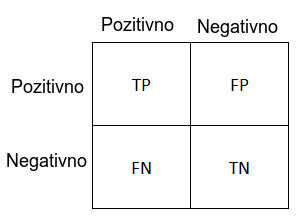
\includegraphics[width=7cm]{slika12}
	\caption{Matrica zabune \protect\footnotemark}
\end{figure}

\footnotetext{https://revolution-computing.typepad.com/.a/6a010534b1db25970b01bb08c97955970d-pi}

Za popunjavanje matrice potrebno je za svaku klasu odrediti broj: ispravno pozitivnih primjera (engl. \textit{true positivie, TP}), lažno pozitivnih primjera (engl. \textit{false positive, FP}), ispravno negativnih primjera (engl. \textit{true negative,TN}) te lažno negativnih primjera ( engl. \textit{false negative,FN}). 

Ispravno pozitivni primjeri su svi pozitivni primjeri za koje je i klasifikator rekao da su pozitivni, lažno pozitivni primjeri su svi negativni primjeri za koje je klasifikator rekao da su pozitivni, ispravno negativni primjer su negativni primjeri za koje je klasifikator rekao da su negativni te lažno negativni primjeri su svi pozitivni primjeri za koje je klasifikator rekao da su negativni. \newline

U ovom radu primarni fokus prilikom evaluacije rezultata je na metriku točnosti, odnosno gledano je samo koliki je broj primjera klasifikator pogodio točno.
 
Točnost (engl. \textit{accurracy}) je opisana kao omjer između ispravno pogođenih primjera i ukupnog broja primjera.
 
 	$$\textit{Acc} = \frac{TP + TN}{TP+TN+FP+FN}$$ \newline
 	
\section{Određivanje spola autora}

Prvi model je binarna klasifikacija spola. Na temelju \textit{tvita} model treba predvidjeti pripada li taj \textit{tvit} autoru ili autorici. Početna raspodjela autora po spolu prikazana je u tablici 5.1.\newline

\begin{table}[h!]
	\centering
	\begin{tabular}{||c |c | c||} 
		\hline
		Skup podataka & Muško & Žensko \\ [0.5ex] 
		\hline\hline
		Trening & 76 & 76 \\ 
		Test & 35 & 35  \\
		\hline
	\end{tabular}
	\caption{Raspodjela broja autora po spolu}
	\label{Table:1}
\end{table}

U sklopu ovog modela korišteni su SVM i logistička regresija. Nakon što su odabrani algoritmi strojnog učenja, provedeni su optimizacijski testovi nad svakim modelom. Odabir optimalnog hiperparametara proveden je pretragom kroz spektar eksponencija broja dva u potrazi za optimalnim hiperparametrom C. Za optimizaciju modela je korišten, već prije spomenuti, skup za provjeru. 

U ovom modelu korištena su oba skupa značajki. Prvo je istrenirana verzija sa skupom značajki sadržaja teksta te zatim zajedno sa skupom značajki stila kako bi se dobio kumulativni utjecaj značajki na prediktivnu moć modela. Model je istreniran na skupu za učenje te testiran na skupu za testiranje. 

Za referentni model spolne klasifikacije je korišten klasfikator većinske klase (engl. \textit{majority class classifier, MCC}) koji predviđa samo klasu koja je u većini. U slučaju spola radi se o ravnomjernoj podijeli te je stoga preciznost modela 50\%.

\newpage

\subsection*{Određivanja spola autora korištenjem značajka sadržaja teksta}

Rezultati binarne klasifikacije autora prema spolu pri korištenju samo skupa značajki sadržaja teksta prikazan je u tablici 5.2.

\begin{table}[h!]
	\centering
	\begin{tabular}{||c|c||} 
		\hline
		Model & Točnost\\ [0.5ex] 
		\hline
		Referentni model & 0.500\\
		\hline
		SVM+Word2Vec & 0.604 \\
		\hline
		SVM+Glove & 0.610 \\
		\hline
		\textbf{SVM+fastText} & \textbf{0.611} \\
		\hline 
		Logistic+Word2vec & 0.600 \\ 
		\hline
		Logistic+GloVe & 0.611 \\ 
		\hline
		Logistic+fastText & 0.609 \\ 
		\hline
	\end{tabular}
	\caption{ Rezultate klasifikacije spola uz korištenje samo skupa značajki sadržaja teksta}
	\label{Table:1}
\end{table}


Na temelju tablice 5.2 vidimo kako je razlika točnosti među algoritmima neprimjetna te da vrsta klasifikatora, u ovom zadatku, ne utječe mnogo na samu točnost modela. Osim algoritma strojnog učenja, na točnost modela također ne utječe način na koji su dobivene značajke sadržaja teksta. Primijetimo da je razlika među alatima za vektorsku reprezentaciju riječi također relativno malena te u nekim situacija i neznatna.\newline


\begin{equation}
	\begin{bmatrix}
	4342 & 2568 \\
	2482 & 3786
	\end{bmatrix}
\end{equation}\newline

Matrica zabune 5.1 prikazuje evaluacijsku procjenu rezultata numerički najboljeg modela iz tablice 5.2 (\textbf{SVM + fastText}). Iz matrice možemo primijetiti kako model može relativno kvalitetno diferencirati muške i ženske autore, no također brojevi lažno pozitivnih i negativnih primjera su također u relativno jednakom omjeru te time zaključujemo da model može uistinu dobro razlikovati spol autora, no isto toliko često i griješi u svojoj procjeni.


\newpage

\subsection*{Određivanje spola autora korištenjem značajka sadržaja i autora teksta}

Rezultati binarne klasifikacije autora prema spolu pri korištenju skupa značajki sadržaja i autora teksta je u tablici 5.3.


\begin{table}[h!]
	\centering
	\begin{tabular}{||c|c||} 
		\hline
		Model & Točnost\\ [0.5ex] 
		\hline
		Referenti model & 0.500\\
		\hline
		\textbf{SVM+Word2Vec+stilometrija} & \textbf{0.632} \\
		\hline
		SVM+Glove+stilometrija & 0.630 \\
		\hline
		SVM+fastText+stilometrija & 0.629 \\
		\hline 
		Logistic+Word2vec+stilometrija & 0.621 \\ 
		\hline
		Logistic+GloVe+stilometrija & 0.619 \\ 
		\hline
		Logistic+fastText+stilometrija & 0.618 \\ 
		\hline
	\end{tabular}
	\caption{ Rezultate klasifikacije uz korištenje samo skupa značajki sadržaja teksta}
	\label{Table:1}
\end{table}

Na temelju tablice 5.3 vidimo kako su se uistinu mjere točnosti povećale sa dodavanjem stilometrijskih značajki. No, rast je relativno malen i s obzirom na početne vrijednosti iz tablice 5.2, vidimo kako je model sa word2vecom preuzeo ulogu najtočnijeg, a model sa fastTextom je postao objektivno najlošiji model.\newline

\begin{equation}
\begin{bmatrix}
4741 & 2169 \\
2702 & 3566
\end{bmatrix}
\end{equation}\newline

Iz matrice 5.2 vidimo kako je u odnosu na matricu 5.1 broj ispravno pogođenih primjera porastao, no omjeri su i dalje relativno jednaki te je broj lažno pozitivnih i negativnih primjera ostao približno  isti. Primijećeni mali porast u točnosti moguće je objasniti sa upotrebom neadekvatnih stilometrijskih značajki za ovaj tip profiliranja. Značajke koje su korištene jednostavno nisu dovoljno specifične kako bi dovoljno razdvojile muško i ženski stil tvitanja. U radu \citep{rangel2013} pokazano je kako uistinu postoje stilometrijske značajke koje su specifične za pojedine spolove, no u ovom radu nisu korištene takve značajke.

\newpage
\subsection*{Zaključak o određivanju spola autora}

S obzirom na dobivene rezultate možemo zaključiti da oba skupa značajki donose svoj doprinos pri povećanju prediktivne moći modela. Skup značajki sadržaja teksta nam je demonstrirao kako značajke sadržaja teksta uistinu mogu pomoći pri klasifikaciji spola autora, no također otkrivamo kako način na koji reprezentiramo  riječi ne donosi veliku razliku. S druge strane, stilometrijske značajke nisu puno povećale točnost modela te se sumnja na pogrešan izbor stilometrijskih značajki za ovaj tip klasifikacije. Značajke korištene u ovom radu više su fokusirane na gramatičku kvalitetu teksta i pismenost autora, a klasifikacija spola zahtijeva značajke koje su više fokusirane na specifičnosti muških i ženskih stilova izražavanja. Značajke poput broja korištenih prijedloga i/ili usklika za koje eksperimenti pokazuju da pozitivno utječu na prediktivnu moć spolnih klasifikatora \citep{rangel2013}. Numerički najbolji model za binarnu klasifikaciju spola je ispao SVM uz word2vec i deset stilometrijskih značajki.


\section{Određivanje dobi autora}

Drugi model je određivanje dobi autora na temelju njegovih ili njezinih objava na Twitteru. Dob se klasificira u četiri klase: 18-24, 25-34, 35-49 i 50-xx. Ovakva podijela dobi povlači se iz činjenice da su većina korisnika interneta mladi te se želi vidit postoje li dovoljno jasne stilske razlike među mlađim dobnim skupinama za kvalitetno profiliranje autora.

 U sklopu ovog modela korišteni su SVM i logistička regresija, ali s podešenim parametrima za višeklasnu (engl. \textit{multiclass}) klasifikaciju. Kao i u prvom modelu, provedena je optimizacija hiperparametra algoritma uz unakrsnu validaciju (engl. \textit{cross-validation}) na skupu za provjeru.

Za ovaj model su također korištena dva skupa značajki: značajke usmjerene na zahvaćanje sadržaja teksta i značajke usmjerene na zahvaćanje stila autora. Raspodjela autora po dobi u skupovima podataka prikazana je u tablici 5.4.\newline

Za referentni model dobne klasifikacije korišten je također klasfikator većinske klase (engl. \textit{majority class classifier, MCC}) te je u slučaju dobne klasifikacije imao preciznost od 40.8\%. Najbrojnija dobna klasa je bila 18-24. 


\begin{table}[h!]
	\centering
	\begin{tabular}{||c |c |c| c| c||} 
		\hline
		Skup podataka & 18-24 & 25-34 & 35-49 & 50-xx \\ [0.5ex] 
		\hline\hline
		Trening & 60 & 58 & 22 & 12 \\ 
		\hline
		Test & 29 & 28 & 10 & 4 \\
		\hline
	\end{tabular}
	\caption{Raspodjela broja autora po dobi}
	\label{Table:1}
\end{table}

\newpage

\subsection*{Određivanje dobi autora korištenjem značajki sadržaja teksta}

Rezultati višestruke klasifikacije autora prema dobi pri korištenju skupa značajki za zahvaćanje sadržaja teksta prikazani su u tablici 5.5.

\begin{table}[h!]
	\centering
	\begin{tabular}{||c|c||} 
		\hline
		Model & Točnost\\ [0.5ex] 
		\hline
		Referentni model & 0.408\\
		\hline
		SVM+Word2Vec & 0.585 \\
		\hline
		SVM+Glove & 0.542 \\
		\hline
		\textbf{SVM+fastText} & \textbf{0.603} \\
		\hline 
		Logistic+Word2vec & 0.578 \\ 
		\hline
		Logistic+GloVe & 0.539 \\ 
		\hline
		Logistic+fastText & 0.594 \\ 
		\hline
	\end{tabular}
	\caption{ Rezultate višeklasne klasifikacije dobi uz korištenje samo skupa značajki sadržaja teksta}
	\label{Table:1}
\end{table}

Iz tablice 5.5 primjećujemo kako za razliku od klasifikacije spola utjecaj različitih alata za vektorsku reprezentaciju riječi nosi puno veću težinu. Iako i različiti klasifikatori donosi različite rezultate, razlike su relativno male.
Zbog povećih razlika pri korištenju GloVe i fastText alata, zaključujemo da način na koji reprezentiramo riječi nosi značajniju ulogu u klasifikaciji dobi korisnika Twitter.\newline

\begin{equation}
\begin{bmatrix}
4064 & 1170 & 24 & 0 \\
1552 & 3695 & 96 & 0 \\
353 & 1343 & 153 & 0\\
329 & 361 & 38 & 0\\
\end{bmatrix}
\end{equation}\newline

Iz matrice zabune 5.3 možemo vidjeti kako je model pristran prema mlađoj populaciji te da nikada ne pogađa zadnju klasu \textit{50-xx}. Najveći broj ispravnih klasa ima prva klasa \textit{18-24}, no ta klasa ima i ujedno najveći broj primjera u skupu podataka. Na temelju svih dobivenih rezultata možemo zaključiti da sadržaje značajki teksta imaju ulogu u klasifikaciji dobi, no model postaje pristran najbrojnijoj klasi te nije u stanju kvalitetno razlikovati određene dobne kategorije.



\subsection*{Određivanje dobi autora korištenjem značajki sadržaja i autora teksta}


Rezultati višeklasne klasifikacije autora prema dobi pri korištenju skupa značajki za zahvaćanje sadržaja teksta i skupa značajki za zahvaćanje stila autora teksta prikazani su u tablici 5.6.

\begin{table}[h!]
	\centering
	\begin{tabular}{||c|c||} 
		\hline
		Model & Točnost\\ [0.5ex] 
		\hline
		Referentni model & 0.408\\
		\hline
		SVM+Word2Vec+stilometrija & 0.635 \\
		\hline
		SVM+Glove+stilometrija & 0.601 \\
		\hline
		\textbf{SVM+fastText+stilometrija} & \textbf{0.641} \\
		\hline 
		Logistic+Word2vec+stilometrija & 0.630 \\ 
		\hline
		Logistic+GloVe+stilometrija & 0.597 \\ 
		\hline
		Logistic+fastText+stilometrija & 0.618 \\ 
		\hline
	\end{tabular}
	\caption{ Rezultate klasifikacije uz korištenje samo skupa značajki sadržaja teksta}
	\label{Table:1}
\end{table}

Na temelju rezultata tablice 5.6. vidimo kako je utjecaj stilometrije na dobnu klasifikaciju mnogo snažniji. Utjecaj klasifikatora je i dalje jednako neznatan, a najdominantniji alat za reprezentaciju riječi i dalje ostaje fastText.

\begin{equation}
\begin{bmatrix}
4531 & 650 & 43 & 0 \\
1245 & 3694 & 290 & 20 \\
138 & 1657 & 29 & 25\\
296 & 296 & 0 & 136\\
\end{bmatrix}
\end{equation}\newline

Iz matrice zabune 5.4. dobivamo zanimljive informacije. Naime, nakon uvođenja skupa stilometrijskih značajki točnost se znatno povećala, no također uočavamo kako je matrica malo bolje distributirana te da model počinje bolje uočavati razlike između pojedinih dobnih klasa. Analizirajući tablicu malo bolje, možemo uočiti kako druga i treća dobna klasa imaju približno iste distribucije, dok je četvrta klasa sličnija distribuciji prve klase. To nas navodi na zaključak da stil pisanja između druge klase (\textit{25-34}) i treće klase (\textit{35-49}) relativno sličan, dok je stil pisanja prve, te djelomično četvrte, klase dovoljno specifičan da ga model gotovo uvijek može raspoznati.



\subsection*{Zaključak o određivanju dobi autora}

Rezultati eksperimenata za dobnu klasifikaciju demonstrirali su nekoliko stvari. Prvenstveno, uočeno je kako u dobnoj klasifikaciji vrsta klasifikatora igra znatno značajniju ulogu. Također, primijećeno je kako način reprezentacije riječi više utječe na točnost, nego kod spolne klasifikacije. Velika razlika u odabiru klasifikatora te vrsti značajki sadržaja teksta upućuje na veću raznolikost stilova pisanja u različitim dobnim skupinama. S druge strane, stilometrijske značajke znatno povećavaju točnost modela. Skup značajki stila prilagođen je i napravljen prvenstveno za detekciju razlike u kvaliteti pisanja te razinu pismenosti autora. S obzirom na povećanje točnosti i bolju  redistribuciju matrice zabune, zaključujemo kako su stilometrijske značajke, s naglaskom na značajke kvalitete teksta i pismenost, povezane uz određene dobne parametre te da pozitivno utječu na dobnu klasifikaciju autora. Također, dubljom analizom rezultata možemo zaključiti da tako dobra distribucija prve i druge dobne skupine upućuje na visoku specifičnost stilskog izražavanja mlađih dobnih skupina te korelacijsku vezu između značajki kvalitete teksta i pismenosti autora s mladenačkim načinom izražavanja. Objektivno najbolji model za višestruku klasifikaciju dobi je bio SVM uz fastText i deset stilometrijskih značajki.

\newpage



\section{Određivanje intenziteta karakternih značajki autora}

Zadnji model je za određivanje intenziteta karakternih značajki autora. Radi se o pet karakternih značajki: \textit{ekstrovertnost, stabilnost, otvorenost, savjesnost i ugodnost} (engl. \textit{extrovertness, stable, open, conscientious, agreeable}). Odabir ovih pet karakternih značajki je usko vezan uz poznati peterofaktorski model osobnosti(engl. \textit{big five personality traits}) koji opisuje pet značajka kao temelje osobnosti.\footnote{https://en.wikipedia.org/wiki/Big\_Five\_personality\_traits}

Za svaku od značajki potrebno je predvidjeti koji intenzitet značajke autora ima. Intenzitet se uzima kao diskretna vrijednost u intervalu od -0.5 do 0.5.  U ovom modelu koristimo SVM-ovu regresiju te predviđene kontinuirane vrijednosti zaokružujemo na jednu od diskretnih vrijednosti ponuđenog spektra. Zaokružene vrijednosti zatim uspoređujemo sa stvarnim vrijednostima te koristimo standardnu mjeru točnosti kao evaluacijsku mjeru rezultata. Za ovaj model su također korištena dva skupa značajki: skup značajki usmjerene za zahvaćanje sadržaja teksta i skup značajki usmjerene za zahvaćanje stila autora. Referentni model u ovome zadatku bio je također klasifikator većinske klase. Sve klase su bile ravnomjerno redistributirane za svaku značajku te je stoga preciznost u ovom slučaju svega 9\%.  


\subsection*{Određivanje intenziteta karakternih značajki autora korištenjem značajki sadržaja teksta}

Rezultati određivanja intenziteta karakternih značajki regresijom te zaokruživanjem na diskretne vrijednosti uz korištenje skupa značajki koje zahvaćaju sadržaj teksta prikazani su u tablici 5.7.

\begin{table}[h!]
	\centering
	\begin{tabular}{||c | c | c | c | c | c||} 
		\hline
		& Ekstrovertnost & Stabilnost & Otvorenost & Savjesnost & Ugodnost \\ [0.5ex] 
		\hline\hline
		Referentni model & 0.09 & 0.09 & 0.09 & 0.09 & 0.09 \\
		\hline
		SVM+Word2Vec & 0.229 & 0.137 & 0.155 & 0.161 & 0.216 \\
		\hline
		SVM+Glove & 0.230 & \textbf{0.199} & \textbf{0.159} & 0.160 & 0.212 \\
		\hline
		SVM+fastText & \textbf{0.234} & 0.137 & 0.134 & \textbf{0.171} & \textbf{0.220} \\
		\hline 
	\end{tabular}
	\caption{Rezultate određivanja intenziteta karakternih značajki uz korištenje skupa značajki sadržaja teksta}
	\label{Table:1}
\end{table}

Iz tablice 5.7 primjećujemo da utjecaj reprezentacijskih alata znatno utječe na točnost određivanja intenziteta psiholoških značajki. U radu objavljenom u sklopu PAN 2015 spomenuto je kako je značajka s najlošijim rezultatima bila stabilnost, za koju se vjeruje da treba visoku dozu kontekstualnog razumijevanja teksta te da je teško iz semantičkih značajki odrediti autorovu stabilnost \citep{notebook2015}. U ovom slučaju primjećujemo da stabilnost pokazuje znatno poboljšanje prilikom korištenja alata GloVe za reprezentaciju u odnosu na word2vec i fastText. GloVe je poznat po svojem specifičnom načinu reprezentacije riječi koji ovdje možda dolazi do izražaja te zbog toga dobivamo kvalitetnije rezultate. Osim stabilnosti, GloVe je najbolji i za otvorenost, dok je fastText najbolji u svim ostalim značajkama.


\subsection*{Određivanje intenziteta karakternih značajki autora korištenjem značajki sadržaja i autora teksta}

Rezultati određivanja intenziteta karakternih značajki regresijom te zaokruživanjem na diskretne vrijednosti, uz korištenje skupa značajki koje zahvaćaju sadržaj teksta i skupa značajki koje zahvaćaju stil autora teksta, prikazani su u tablici 5.8.

\begin{table}[h!]
	\centering
	\begin{tabular}{||c | c | c | c | c | c|c||} 
		\hline
		& Ekstrovertnost & Stabilnost & Otvorenost & Savjesnost & Ugodnost \\ [0.5ex] 
		\hline\hline
		Referentni model & 0.09 & 0.09 & 0.09 & 0.09 & 0.09  \\
		\hline
		SVM+w2v+stil & 0.261 & 0.142 & 0.186 & 0.181 & \textbf{0.258}  \\
		\hline
		SVM+GloVe+stil & 0.253 & \textbf{0.208} & \textbf{0.189} & 0.177 & 0.246  \\
		\hline
		\textbf{SVM+fastText+stil} & \textbf{0.268} & 0.144 & 0.171 & \textbf{0.220} & 0.257 \\
		\hline
	\end{tabular}
	\caption{Rezultate određivanja intenziteta karakternih značajki uz korištenje skupa značajki sadržaja i autora teksta}
	\label{Table:1}
\end{table}

Iz tablice 5.8 vidimo da su najbolji modeli ostali isti, uz iznimku ugodnost gdje je sada najtočniji model \textit{SVM+w2v+stil}. Analizirajući dodatno rezultate zaključujemo kako stilometrijske značajke dodaju određeno poboljšanje, no u odnosu na referentne modele iz tablice 5.7 vidimo kako je utjecaj malen i prigušen već relativno visokom točnošću referentnih modela. Na temelju već obrađenih radova s ovim tipom zadataka, otkrivamo kako je određivanje intenziteta prilično kompleksan i zanimljiv problem koji zahtijeva dobro promišljene značajke \citep{rangle2015}. Pojedine osobine poput stabilnosti i savjesnosti su iznimno kompleksne psihološke značajke koje traže visoku razinu kompleksnosti u značajkama s kojima ih detektiramo. S druge strane, značajke ekstrovertnosti i ugodnosti puno su izraženije kroz prirodni jezik te ih je puno lakše detektirati stilskim i sadržajnim značajkama. Objektivno najuspješniji model za ovaj problem bio je SVM uz fastText i deset stilometrijskih značajki.


\newpage

\subsection*{Zaključak o određivanju intenziteta karakternih značajki autora}
 
Rezultati eksperimenata određivanja intenziteta psiholoških značajki nose sa sobom nekoliko zaključaka. Prije svega uočavamo kako je skup značajki sadržaja postavio relativno visoke točnosti te da različiti načini reprezentacije riječi ponovo imaju visoki utjecaj na samu točnost modela. S druge strane, stilometrijske značajke donijele su relativno nisko poboljšanje modela. Zaključujemo da je skup stilometrijski značajki neprikladan za ovaj tip problema te da je potrebno isprobati ove modele sa značajkama koje će adekvatnije specificirati stilske razlike potrebne za kvalitetnije određivanje intenziteta psiholoških značajki. Objektivno najuspješniji model za ovaj problem bio je SVM uz fastText i deset stilometrijskih značajki.



\chapter{Zaključak}

U svijetu prepravljenom društvenim mrežama svakodnevno raste interes za sve kvalitetnijim i temeljitijim profiliranje sve većeg broja korisnika i objava. Sve veći broj podataka i korisnika zahtijeva promišljeni pristup i pomoć računalnih resursa. Grana računarske znanosti koja se bavi ovakvim problemima naziva se profiliranje autora. Kod zadatka profiliranja autora radi se na determiniranju određenih demografskih obilježja autora poput dobi, spola te ostalih značajka poput osobnosti.

U ovom radu željelo se uspješno demonstrirati uspješnost klasifikacije doba i spola uz dodatan zadatak određivanja intenziteta  psiholoških značajki autora. Izgrađena su tri modela za koja su redom pripremljena dva različita skupa značajki. Prvi skup značajki su značajke sadržaja teksta za koje se koristila vektorska reprezentacija riječi (engl. \textit{word embeddings}). Korištena su tri najpopularnija alata za vektorsku reprezentaciju, a to su redom Word2vec, GloVe (engl. \textit{Global Vectors}) i fastText. Drugi skup značajki su značajke stilometrije čiji cilj je zahvaćanje stila autora. Značajke koje su korištene su prikupljene iz srodnih radova \citep{rangel2013} i \citep{rangle2015}. Preuzete značajke bile su fokusirane na detekciju kvalitete teksta i svojevrsne pismenosti autora. Najuspješniji model kroz sve zadatke se pokazao kao spoj SVM-a uz fastText i deset izabranih stilometrijskih značajki. Rezultati spolne klasifikacije spola iznosili su 63.2\%, dok je za klasifikaciju dobi najbolji model imao točnost od 64.1\%. U zadatku s određivanjem intenziteta psiholoških značajki bilo je razmatrano pet modela SVM-regresije od kojih je najbolji imao točnost 26.8\% za značajku ekstrovertnosti.  

U budućim radovima trebalo bi se usmjeriti na kvalitetnije razvijanje stilometrijskih značajki za tip zadataka na kojem se primjenjuju. Značajke koje su se prilagodile prirodi zadataka pokazale su znatno veću preciznost i točnost u modelima koji su ih koristili \citep{rangle2015}. U ovom radu ograničili smo se na određen tip stilometrijskih značajki te smo zbog toga na klasifikaciji spola i određivanju intenziteta psiholoških značajki postigli slabije rezultate no što je bilo očekivano.

\bibliography{literatura}
\bibliographystyle{fer}

\begin{sazetak}

Profiliranje autora metoda je analize tekstova kod kojega se na temelju autorovog teksta otkrivaju određene informacije o autoru. Metode za profiliranje autora većinom se oslanjaju na stilometrijska obilježja teksta te su zbog toga izrazito korisne u današnjem svijetu obilježenom velikom brojem društvenih mreža. Ovaj rad se bavi određivanjem spola, dobi te intenziteta psihološki značajki autora. Modeli su temeljeni na alatima obrade prirodnog jezika i algoritmima strojnog učenja. Nakon razvoja modela za određivanje spola,dobi i intenziteta psiholoških značajki autora, provedeno je i eksperimentalno vrednovanje modela i analiza dobivenih podataka.


\kljucnerijeci{obrada prirodnog jezika, profiliranje autora, društvene mreže,  strojno učenje.}
\end{sazetak}

% TODO: Navedite naslov na engleskom jeziku.
\engtitle{Author Profiling of Social Media Users}
\begin{abstract}
	Author profiling is a method of analyzing a given number of texts to try to uncover various characteristics of the author.
	Profiling methods are largely based on the stylometric features of the text and are therefore extremely useful in today's world marked by a large number of social networks. This paper deals with the determination of gender, age, and intesity of psychological features of the author. The models are based on natural language processing tools and machine learning algorithms. After the development of gender, age and intesity of psychological features models, experimental evaluation of the model and analysis of the obtained data was performed.

\keywords{natural language processing, author profiling, social network, machine learning.}
\end{abstract}

\end{document}
